\section{Methodology}


\subsection{Test Environment}
In our experiments, we were using the ODROID-X2 \cite{odroid-x2} developer
platform, which has an Exynos 4412 "Prime" System-on-Chip with four ARM
Cortex-A9 (r3p0) processor cores. We disable CPU core 1 through 3, leaving only
one core configured to run at a static frequency of $1.7$ GHz.

The Cortex-A9 is a 32-bit out-of-order dual-issue speculative RISC processor
with many features common for modern processor designs\cite{patterson}\cite{hennessy},
making it attractive for our experiments. After the dispatch stage, its pipeline
is split into four different lanes, each with its own functional units.
Documentation on the internal structure of the pipelines are not publicly
available, but by running experiments similar to the ones presented in
\cite{bircher}\cite{bertran}\cite{singh}  (explained below) and looking at previous
work regarding and existing techncal details\cite{armtech}\cite{7cpu}, we are able to infer some
details.  The four pipelines are structured as follow: Main execution pipeline
with a general ALU, and a hardware-multiply, secondary execution pipeline with
only a general ALU, load-store-pipeline, containing only an hardware adder to
generate addresses, and a floating-point pipeline containing an ordinary FPU and
connections to the NEON unit. See \autoref{fig:pipeline}.

\begin{figure}
    \begin{centering}
        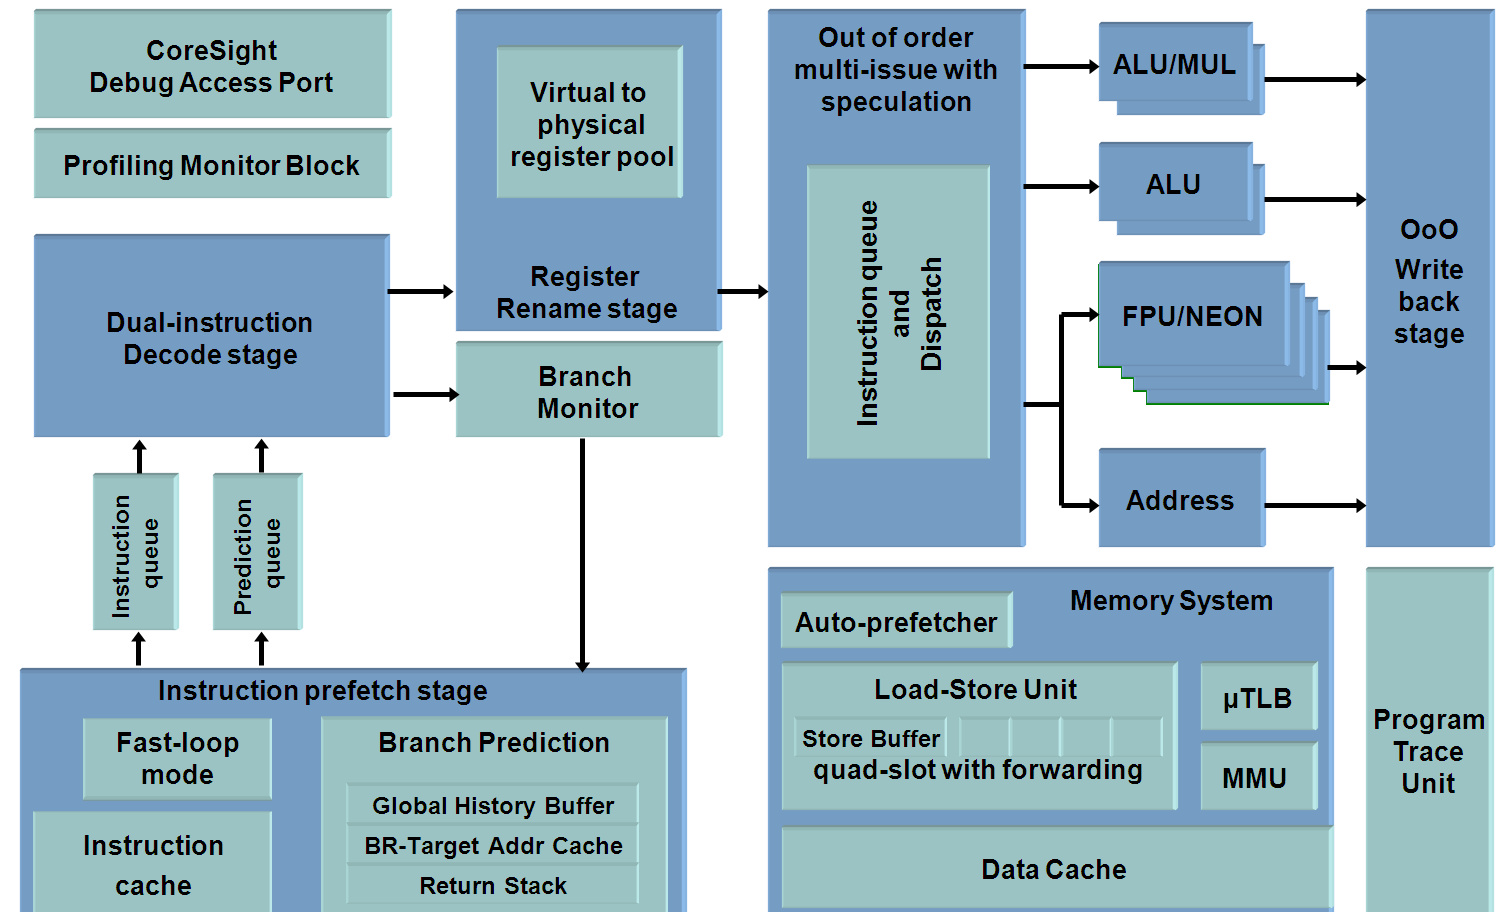
\includegraphics[width=0.48\textwidth]{figures/A9-Pipeline-hres}
        \caption{ARM Cortex-A9 Pipeline and peripherals,\hfill
        figure from ARM Cortex-A9 Whitepaper\cite{a9whitepaper}}
        \label{fig:pipeline}
    \end{centering}
\end{figure}

\subsection{Architectural Experiments}
\label{arch_experiments}
Because the energy efficiency is often different at different amounts of
workload, we seek to stress the processor as much as possible when we run our
tests. In order to run the processor at it's highest possible throughput, it is
required that we gain some knowledge of it's pipeline and other components
within the CPU. As we are using a proprietary platform as our target
architecture, only some of these details are known. Thus, we define test
programs to stress particular pipeline components and gather statistics using
performance counters. By comparing execution unit counters and the total cycle
count, we obtain detailed (although approximate, due to the speculativity in the
core) information of a test program's execution. \todo[inline]{Elaborate in
detail, see notes/alu-count.txt.}

The A9 processor has 58 distinct events that each can be mapped to one of six
generic event counters in the Performance Monitor Unit (i.e. only six generic
events can be tracked simultaneously). It also has a separate cycle counter. A
complete overview can be seen in table $A.18$ in the Cortex-A9 Technical
Reference Manual \cite{armtech}.

Using performance counters as above, we are able to confirm a feature on the A9
processor that is very vaguely documented; fast-loop\texttrademark mode. As the
name suggests, this feature enables rapid execution of small loops. It does so
by fetching from the instruction cache only at the first loop iteration,
effectively voiding time and energy spent on instruction cache lookups between
iterations. However, which loops that falls into this category is not
documented, but by using performance counters we are able to determine this with
confidence.
\todo[inline]{Add appendix explaining fast-loop microbenchmark.}

Furthermore, executing code within fast-loop limits the number of cache
mispredicts to 2 independently of the iteration count. We confirm this by
looking at the cache mispredict \todo[inline]{name?} performance counter. The first miss
is likely to occur at the end of the first iteration, while the second occurs on
the way out of the loop.

\subsection{Benchmarks}
As a first approximation, the benchmark programs consists of an infinite series
of identical instructions. The A9 core runs at a fixed frequency and we are
providing a fixed core voltage, so energy usage of simple, one-cycle instruction
could be retrieved by running for a fixed time period and applying the following
formula.

\todo[inline]{fix formula}
\begin{equation}
    P_{instruction} = A_{instruction} \cdot V_{core}
\end{equation}
\begin{equation}
    E_{instruction} = P_{instruction} \cdot CPI_{instruction}
\end{equation}


This simple setup does not take the memory system into account; we are
undoubtedly not able to feed the processor instructions at no cost in terms of
access speed and -- more importantly -- memory system energy usage. Thus, we
enhance our setup by running all benchmark code within fast-loop, as explained
above.


\begin{figure}
    \begin{lstlisting}{language=[ARM]Assembler}
    label: instruction
    ... (repeats 13X)
    instruction
    subs
    jne label
    \end{lstlisting}
    \caption{Instruction loop}
    \label{list:inst_loop}
\end{figure}

The technical manual states that branching to immediate locations does not
consume execution unit cycles. Our microbenchmarks branches to immediate
locations, but it does so only when a certain condition is met. We assume that
the calculation of this condition takes normal execution time, but that the
branch is invisible.


\subsection{Power Measurements}
To measure energy consumption, we use an Agilent 34410A
multimeter\cite{agilent34410a} and measures voltage drop over a negligible $12$
$m\Omega$ resistor. The multimeter is set to sample at full precision at its
maximum rate of 1000 Hz. This gives one sample every 1.7 million instructions
with an error of at most 0.002V. It is obvious that we are unable to observe
inter-cycle fluctations, but as we run the same instruction practically
indefinetely we get an average.

We decouple power consumption on the ARM cores and the development board by
modifying the ODROID-X2 and providing a separate power supply for the A9 cores.
They get powered by an external power supply giving $1.3V$ DC, while the rest of
the board is powered from a another power supply at $5.0V$, as depicted in
figure \ref{fig:setup}.

\subsection{Pitfalls}
% temperature, noise (inducted power, etc.), interrupts, memory latency
% (fast-loop)
Since we are comparing the energy efficiency of different instruction in an
asynchronous way, we have to consider factors that affects power usage, as well
as acknowledge that they may differ between runs.

One obvious such factor is temperature, both ambient and the chip temperature.
The first may change without our notice, and the second one is determined by the
ambient, the cooling device and what load tasks that was just run on the SoC. On
this specific SoC, Samsung Exynos 4412, we have detected that the difference
from the CPU Thermal Zone 0 being 9$^\circ$ Celsius and 63$^\circ$ Celsius is on
average between 2-4\%. We also detected that some instructions might have as
much as 7\% higher energy consumption when running at the hotter
level\footnote{This was detected with at the {\ttfamily mul}-instruction}. We
have also checked that running a single core at maximum performance over time
does not increase the temperature by more than from idle at 47$^\circ$ Celsius
to 54$^\circ$ Celsius at load. Assuming that it is generally true that a single
core cannot heat the entire SoC with any significant amount, and that the
increase in power consumption is at max 10\% over 50$^\circ$ Celsius, we get

\begin{equation}
    P_{inc} = P_{orig} \cdot T_{inc} \cdot \frac{0.10}{50} = P_{orig} \cdot T_{inc} \cdot 0.002
\end{equation}

Believing that this trend is at least close to linear, output will increase by
0.2\% pr.  degree Celsius increased. Also, we start our measurements at least
half a second after the benchmarks have been started, thus there is plenty of
time for the CPU to gain work temperature. In our tests, the time used to get to
work temperature was humanly instant.

Another factor that is not that obvious, but at least equally important, is
power inducted in the measurement circuit. Since wires are often winded up on
the test bench, and lab equipment might contain large metal cores with a great
amount of power running through them, unexpected power might be introduced.

We are running Linux on the chip under test, this gives us a much simpler way of
programming the processor to run our tests. The fact that we run an entire
operating system beneath our benchmark programs implies that there is much going
on that we have no direct controls over.  In order to mitigate the artifacts
originating from the operating system, we disable all the mask cable interrupts.

As explained in section \ref{arch_experiments}, we utilize the fast-loop mode of
the processor to mitigate memory access latency. We disable the L1 cache to
easier detect when we are outside the fast-loop mode, and thus we are certain
that there is no memory access going on.
